\documentclass[11pt, a4paper,onecolumn]{article}
\usepackage{style-1}
\usepackage{multirow} 
\usepackage{graphicx} 
%  Linguistics article environments in LaTeX
%  R.L.H. - EUROTRA PROJECT, Dept. Lang & Ling, University of Essex
%  Mar 16 90
%	Revised Aug 90
%
%
%  Input this file into your source file by putting the LaTeX command
%  `` \input <thisfilename> '' on its first line.
%
% `%' starts a comment !

%%	*********** Macro Definitions **************
%%
% LINGUISTIC ITEM ENVIRONMENT
% Linguistic items (examples, diagrams, trees etc) are normally
% numbered consecutively throughout a linguistic article.

\newcounter{licntr}			% linguistic item counter

% Two commands required in the defintion of a linguistic item
\newcommand{\stepli}{\refstepcounter{licntr}}	% increment
					  	% li counter
\newcommand{\lival}{\thelicntr}			% return value
						% of li
						% counter
%% Now we define the ``linguistic item'' environment for cases where
%% there is just one \item to be displayed e.g. a single sentence
%% First, define the outer environment (which handles the numbering)
\newenvironment{liout}{\small
		\stepli			% step li counter
		\samepage			% prevent page break
		\begin{list}{		% begin definition
			(\lival)\hfill}{} 	% left adjust number
			\samepage
			\item 			% dummy item
		}{ \end{list}}

\newenvironment{liexc}{\small
		\samepage			% prevent page break
		\begin{list}{		% begin definition
			(27)\hfill}{} 	% left adjust number
			\samepage
			\item 			% dummy item
		}{ \end{list}}

%% Now embed a new list in the outer list - to typographical match the
%% ``lis'' environment (where we have alpha-indexed items)
\newenvironment{li}{\small
		\begin{liout} 			% begin outer list
		\begin{list}{\samepage \noindent}{} 	% begin inner
						% list,  prevent page break 
		\item}{				% item
		\end{list} 
		\end{liout}}

\newenvironment{liexcp}{\small
		\begin{liexc} 			% begin outer list
		\begin{list}{\samepage \noindent}{} 	% begin inner
						% list,  prevent page break 
		\item}{				% item
		\end{list} 
		\end{liexc}}



%% Special version of li which does NOT indent material - puts number
%% on line by itself and then (unindented) material below
\newenvironment{li*}{\small
	\stepli
	\samepage				% prevent page break
	\begin{trivlist} \item[] (\lival) \end{trivlist}
	\begin{trivlist} 
	{\samepage \item[]}
	}{\end{trivlist}}					% space
				

% LINGUISTIC ITEMS ENVIRONMENT
% Define a counter for alphabetically indexed items
\newcounter{alphcntr}		% will be reset in each new lis environment

% Define an environment (called ``lis'' = linguistic items) for a
% series of alpha-indexed linguistic items e.g. 
%	(1) a.
%	    b.    etc.
\newenvironment{lis}{\small
		\begin{liout} 				% begin outer list
			\begin{list}{			% begin inner
							% list
				\samepage		% prevent pg breaks
				\alph{alphcntr}.\hfill 	%left-align letter
					}{
				\usecounter{alphcntr}}}{
		\end{list} \end{liout}}

% LINGUISTIC PRINCIPLE COMMAND - \princ
\newtheorem{prin}{Principle}
%%\newtheorem{ax}{Axiom}
%%\newtheorem{fig}{Figure}
\newtheorem{assum}{Assumption}
\newtheorem{defn}{Definition}
% Define any more you want here.....

% Now define a command with two arguments to handle linguistic
% principles.  The command - ``princ'' takes two arguments: the
% first is the name associated with a \newtheorem (e.g. ``prin'') and
% the second  is the text of that principle. (We use a command here
% rather than an  environment due to technical limitations of LaTeX environment
% parameter handling.)
\newcommand{\princ}[2]{\begin{liout} 
			\begin{#1} 
				{#2}
			\end{#1}
			\end{liout}}
			
			
% MACROS FOR PRODUCING LABELLED/UNLABELLED BRACKETS
\newcommand{\lb}{\mbox{$ [ $}}			% unlabelled right
						% bracket 

\newcommand{\rb}{\mbox{$ ] $}}			% unlabelled right
						% bracket 

\newcommand{\llb}[1]{\mbox{$ [_{#1} $}}		% labelled left
						% bracket

\newcommand{\lrb}[1]{\mbox{$ ]_{#1} $}}   	% labelled right
					      	% bracket

% MACROS FOR HANDLING LISTS, SHORTCUTS etc - A.W., 13/1/95
\newcommand{\bi}{\begin{itemize}}		 
\newcommand{\ei}{\end{itemize}}		 

\newcommand{\be}{\begin{enumerate}}		 
\newcommand{\ee}{\end{enumerate}}

\newcommand{\bc}{\begin{center}}		
\newcommand{\ec}{\end{center}}		

\newcommand{ \heading }[1]{ \begin{center}
			   {\bf {#1}}
			    \end{center}}

% MACROS FOR STANDARD LINGUISTIC SYMBOLS (can be used in text mode)
\newcommand{\tarr}{\mbox{$ \Longrightarrow $}}	% ==> i.e
						% translation arrow

\newcommand{\rarr}{\mbox{$ \longrightarrow $}}	% --> i.e.
						% rule arrow

\newcommand{\llr}{\mbox{$ \longleftrightarrow $}}	% <--> i.e.
						% rule arrow

\newcommand{\up}{\mbox{$ \uparrow $}}	% uparrow for text/maths
						% environment

\newcommand{\down}{\mbox{$ \downarrow $}}	% downarrow for
					    	% text/maths environment

%% \newcommand{\th}{\mbox{$ \theta $}}		% theta
\newcommand{\al}{\mbox{$ \alpha $}}		% alpha

% MACROS FOR ASTERISKING LINGUISTIC DATA
% (ensures data strings are neatly aligned e.g
%	Green ideas sleep furiously
%      *Green ideas furious sleep

\newlength{\astspace}				% initialise length command

\settowidth{\astspace}{\mbox{$\ast$}}		% set length command
						% to width of an asterisk

\newcommand{\un}{\mbox{$\ast$}}			% unacceptable string (*)

\newcommand{\qu}{?}				% questionable string

\newcommand{\ac}{\hspace*{\astspace}}		% acceptable string
						% (inserts *-width
						% space at start of
						% string)

%% ATTRIBUTE-VALUE ARRAY ENVIRONMENT		
%% Now we define some specialised linguistic items, starting with an
%% attribute value array
\newcommand{\attrib}[1]{{\rm \bf {#1}}}		% define the
						% attributes of an
						% attribute

\newcommand{\atomval}[1]{{\rm {#1}}}		% define attribute of
						% an atomic value

\newcommand{\sematomval}[1]{{\mit {#1}}}	% define attribute of 
						% semantic atomic values

% Att-Val array environment.  
% Must occur inside maths environment
\newenvironment{av}{\left[ \begin{array}{ll}}{\end{array} \right]}

%% Labelled Att-Val array environment
\newenvironment{lav}[1]{ \left[_{#1} \begin{array}{ll}}{\end{array} \right]}


%% TREE ENVIRONMENT - \begin{tree}{}......\end{tree}
% Trees produced by specialised tabular environment which takes an
% argument corresponding to the width of the tree - a string in c*
% e.g. cccc  for a tree 4 nodes wide. Lines between nodes must be   
% drawn by hand. 
\newenvironment{tree}[1]{		
	\begin{large}				% nodes in large typeface
	\renewcommand{\arraystretch}{4}		% set interrow space
						% to 4 (LaTeX default
						% is 1.  Change this
						% value to increase
						% depth of subtrees.
						% Range 3-6  approx

	\begin{tabular}{{#1}} 			% begin tree with 
						% argument-specified width
	\addtolength{\tabcolsep}{\tabcolsep}	% Double normal table
					    	% column separation. 
	}{				

	\addtolength{\tabcolsep}{-0.5\tabcolsep}	% Restore normal table
					     	% column separation
	\end{tabular}				% end of tree description

	\renewcommand{\arraystretch}{1}		% Restore default
						% array row separation
	\end{large} }				% Back to normal size

%% Commands for drawing boxes around lists, from Arnold et al '94.

\newcommand{\dougswideboxfigure}[3]{	
\begin{figure}[hbtp]
\begin{center}
\begin{tabular}{|p{134mm}|}\hline
%{|@{\hspace{3em}}l@{\hspace{3em}}|}\hline
\\
\multicolumn{1}{|c|}{\bf #2}\\
% only one extra line here is better:\\
\begin{center}
\begin{minipage}[t]{110mm}
#3
\end{minipage}
\end{center}
\\
\hline
\end{tabular}
\end{center}
\label{#1}
\end{figure}
}



\newcounter{figcntr}			% figiom counter

% Two commands required in the defintion of an figiom
\newcommand{\stepfig}{\refstepcounter{figcntr}}	% increment
					  	% fig counter
\newcommand{\figval}{\thefigcntr}		% return value
						% of fig
						% counter

%% Now we define the ``linguistic item'' environment for cases where
%% there is just one \item to be displayed e.g. a single sentence
%% First, define the outer environment (which handles the numbering)
\newenvironment{figout}{
		\stepfig			% step fig counter
		\begin{list}{		% begin definition
			(\figval)\hfill}{} 	% left adjust number
			\item 			% dummy item
		}{ \end{list}}

%% Now embed a new list in the outer list - to typographical match the
%% ``lis'' environment (where we have alpha-indexed items)
\newenvironment{fig}{
		\samepage			% prevent page break
		\begin{figout} 			% begin outer list
		\begin{list}{}{} 		% begin inner list
		\item}{				% item
		\end{list} 
		\end{figout}}

\renewcommand{\thefigcntr}{\Alph{figcntr}}

\newcounter{axcntr}			% axiom counter

% Two commands required in the defintion of an axiom
\newcommand{\stepax}{\refstepcounter{axcntr}}	% increment
					  	% ax counter
\newcommand{\axval}{\theaxcntr}		% return value
						% of ax
						% counter

%% Now we define the ``linguistic item'' environment for cases where
%% there is just one \item to be displayed e.g. a single sentence
%% First, define the outer environment (which handles the numbering)
\newenvironment{axout}{
		\stepax			% step ax counter
		\begin{list}{		% begin definition
			(\axval)\hfill}{} 	% left adjust number
			\item 			% dummy item
		}{ \end{list}}

%% Now embed a new list in the outer list - to typographical match the
%% ``lis'' environment (where we have alpha-indexed items)
\newenvironment{ax}{
		\samepage			% prevent page break
		\begin{axout} 			% begin outer list
		\begin{list}{\noindent}{} 		% begin inner list
		\item}{				% item
		\end{list} 
		\end{axout}}

\renewcommand{\theaxcntr}{\Roman{axcntr}}

%EMBEDDED AXIOMS e.g.
%	(1) a.
%	    b.    etc.

\newcounter{alphacntr}		% will be reset in each new ax environment

\newenvironment{axs}{
		\begin{axout} 				% begin outer list
			\begin{list}{			% begin inner
							% list
				\samepage		% prevent pg breaks
				\alph{alphacntr}.\hfill %left-align letter
					}{
				\usecounter{alphacntr}}}{
		\end{list} \end{axout}}


\newcommand{\s}{\mbox{$ \sectionsymbol $}}      
\let\sectionsymbol=\S
\def\S{{}\;{}}

\usepackage{times}
\usepackage{latexsym}
\usepackage{verbatim}
\usepackage{graphicx}
\usepackage{rotating}
\usepackage[table]{xcolor}


\title{Using Annotations on Mechanical Turk to perform supervised polarity classification of Spanish Customer Comments}

\name{Authors}

\address{Barcelona Media Innovation Center\\
               Av Diagonal 177, 9th floor, 08018 Barcelona \\ 
}
\abstract{
 One of the major bottlenecks in the development of data-driven AI Systems is the cost of reliable human annotations. The recent advent of several crowdsourcing platforms such as Amazon's Mechanical Turk, allowing requesters the access to affordable and rapid results of a global workforce, greatly facilitates the creation of massive training data. Most of the available studies on the effectiveness of crowdsourcing report on English data. We use Mechanical Turk annotations to train an Opinion Mining System to classify Spanish consumer comments. We design three different Human Intelligence Task (HIT) strategies and report high inter-annotator agreement between non-experts and expert annotators. We evaluate the advantages/drawbacks of each HIT design and show that, in our case, the use of non-expert annotations is a viable and cost-effective alternative to expert annotations. \\ \textbf{Keywords:} Annotations on Mechanical Turk, HIT design, supervised polarity classification 
}

\begin{document}


\maketitleabstract

\section{Introduction}
\label{sec:intro}


Obtaining reliable human annotations to train data-driven AI systems is often an arduous and expensive process. For this reason, crowdsourcing platforms such as Amazon's Mechanical Turk\footnote{\texttt{https://www.mturk.com}}, Crowdflower\footnote{\texttt{http://crowdflower.com/}} and others have recently attracted a lot of attention from both companies and academia. Crowdsourcing enables requesters to tap from a global pool of non-experts to obtain rapid and affordable answers to simple Human Intelligence Tasks (HITs), which can be subsequently used to train data-driven applications.

A number of recent papers on this subject point out that non-expert annotations, if produced in a sufficient quantity, can rival and even surpass the quality of expert annotations, often at a much lower cost \cite{snow_cheap_2008}, \cite{su_internet-scale_2007}. However, this possible increase in quality depends on the task at hand and on an adequate HIT design \cite{kittur_crowdsourcing_2008}. 

In this paper, we evaluate the usefulness of AMT annotations to train an Opinion Mining System to detect opinionated contents (Polarity Detection) in Spanish customer comments on car brands. Currently, a large majority of AMT tasks is designed for English speakers. One of our reasons for participating in this shared task was to find out how easy it is to obtain annotated data for Spanish. In addition, we want to find out how useful these data are by comparing them to expert annotations and using them as training data of an Opinion Mining System for polarity detection.

This paper is structured as follows. Section \ref{sect:outline} contains an explanation of the task outline and our goals. Section \ref{sect:design} contains a description of three different HIT designs that we used in this task. In Section \ref{sect:results}, we provide a detailed analysis of the retrieved HITs and focus on geographical information of the workers, the correlation between the different HIT designs, the quality of the retrieved answers and on the cost-effectiveness of  the experiment. In Section \ref{sect:classifier}, we evaluate the incidence of AMT-generated annotations on a polarity classification task using two different experimental settings. Finally, we conclude in Section \ref{sect:conclusions}.

\section{Task outline and goals}
\label{sect:outline} 

We compare different HIT design strategies by evaluating the usefulness of resulting Mechanical Turk (AMT) annotations to train an Opinion Mining System on Spanish consumer data. More specifically, we address the following research questions:\\
 \indent (i) Annotation quality: how do the different AMT annotations compare to expert annotations?\\
 \indent (ii) Annotation applicability: how does the performance of an Opinion Mining classifier vary after training on different (sub)sets of AMT and expert annotations?\\
 \indent (iii) Return on Investment: how does the use of AMT annotations compare economically against the use of expert annotations?\\
 \indent (iv) Language barriers: currently, most AMT tasks are designed for English speakers. How easy is it to obtain reliable AMT results for Spanish? 

\section{HIT design}
\label{sect:design}

We selected a dataset of 1000 sentences containing user opinions on cars from the automotive section of \texttt{www.ciao.es} (Spanish). Ciao is a European based online-shopping portal which contains a forum with user reviews and opinions on a wide variety of products. Figure \ref{ciao} shows an example of the website. 

\begin{figure}[ht]
  \begin{center}
    \fbox{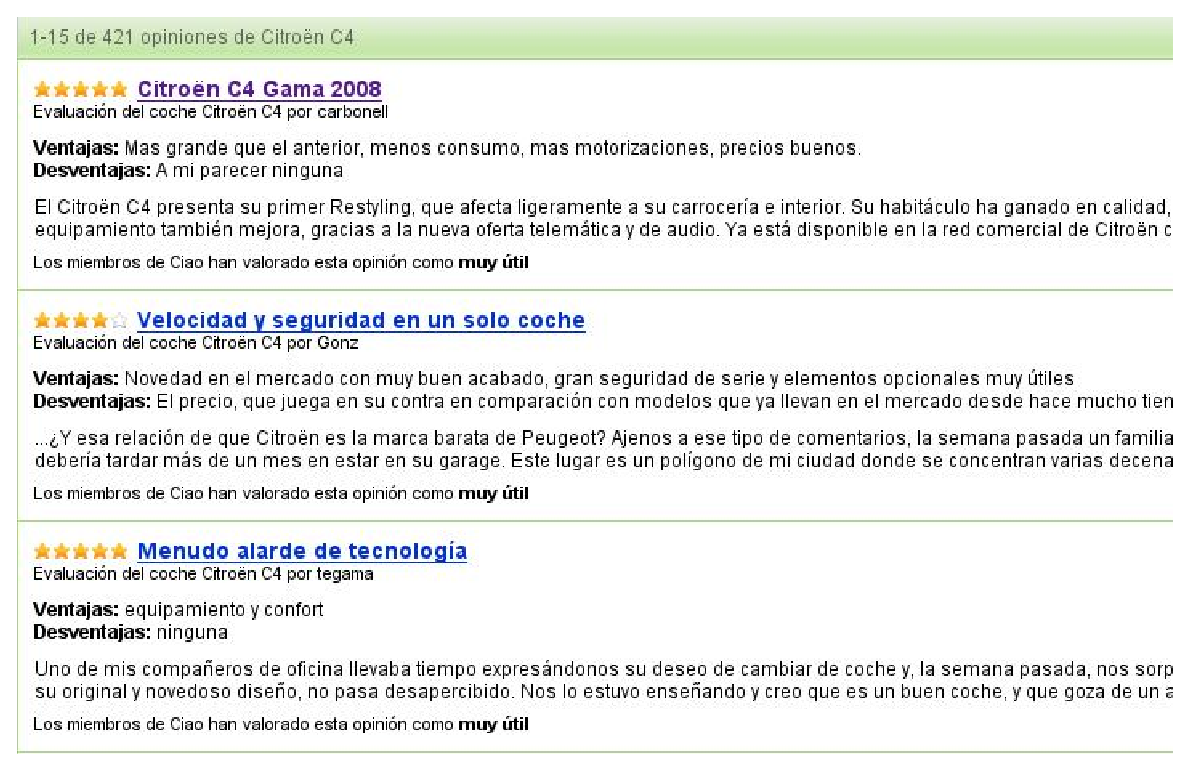
\includegraphics[scale=0.5]{pics/ciao.eps}}
	\caption{Example of the ciao opinions.}
	\label{ciao}
  \end{center}
\end{figure}


This website was chosen because it contains a large and varied pool of Spanish customer comments suitable to train an Opinion Mining System and because opinions include simultaneously global numeric and specific ratings over particular attributes of the subject matter. Section \ref{datasets} contains more detailed information about the selection of the dataset. An example of different sentences from the data set can be found in (\ref{ex}):

\begin{li}
  \label{ex}
  `No te lo pienses m\'{a}s, c\'{o}mpratelo!'\\
  ($=$ `Don't think twice, buy it!')\\
   `Tiene muchas piezas defectuosas'\\
  ($=$ `It contains many defective parts.')\\ 	
   `La conducci\'on es genial pero el dise~no una porquer\'ia'\\
  ($=$ `The car drives great but the design is crap.')\\ 
   `El Volvo es mejor que el Fiat'\\
  ($=$ `Volvo is better than Fiat.')\\ 
 `Este coche tiene 6 cilindros'\\
  ($=$ `This car has 6 cylinders.')\\ 		
\end{li}


The sentences in the dataset were presented to the AMT workers in three different HIT designs. Each HIT design contains a single sentence to be evaluated. 

HIT1 is a simple categorization scheme in which workers are asked to classify the sentence as being either \textit{positive}, \textit{negative} or \textit{neutral}, as is shown in Figure \ref{hit1}. 


\begin{figure}[ht]
  \begin{center}
    \fbox{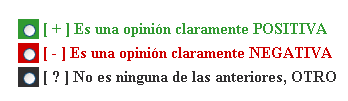
\includegraphics[scale=0.4]{pics/Shot_HIT1.eps}}
	\caption{HIT1: a simple categorization scheme.}
	\label{hit1}
  \end{center}
\end{figure}



HIT2 is a graded categorization template in which workers had to assign a score between -5 (negative) and +5 (positive) to the example sentence, as is shown in Figure \ref{hit2}. 

\begin{figure}[ht]
  \begin{center}
    \fbox{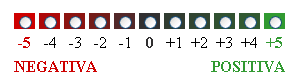
\includegraphics[scale=0.4]{pics/Shot_HIT2.eps}}
	\caption{HIT2: a graded categorization scheme.}
	\label{hit2}
  \end{center}
\end{figure}



Finally, HIT3 is a continuous triangular scoring template that allows workers to use both a horizontal positive-negative axis and a vertical subjective-objective axis by placing the example sentence anywhere inside the triangle. The subjective-objective axis expresses the degree to which the sentence contains opinionated content and was earlier used by \cite{sentiwordnet:06}. For example, the sentence \textit{`I think this is a wonderful car'} clearly marks an opinion and should be positioned towards the subjective end, while the sentence \textit{`The car has six cilinders'} should be located towards the objective end. Figure \ref{hit3} contains an example of HIT3. 

\begin{figure}[ht]
  \begin{center}
    \fbox{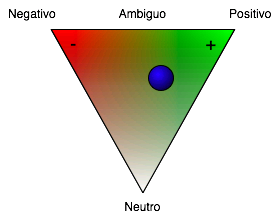
\includegraphics[scale=0.4]{pics/Shot_HIT3.eps}}
	\caption{HIT3: a continuous triangular scoring scheme containing both a horizontal positive-negative axis and a vertical subjective-objective axis.}
	\label{hit3}
  \end{center}
\end{figure}


In order not to burden the workers with overly complex instructions, we did not mention this subjective-objective axis but asked them instead to place ambiguous sentences towards the center of the horizontal positive-negative axis and more objective, non-opinionated sentences towards the lower \textit{neutral} tip of the triangle.

For each of the three HIT designs, we specified the requirement of three different unique assignments per HIT, which led to a total amount of $3 \times 3 \times 1000 = 9000$ HIT assignments being uploaded on AMT. Mind that setting the requirement of unique assigments ensures a number of unique workers \textit{per individual HIT}, but does not ensure a consistency of workers over a single batch of 1000 HITs. This is in the line with the philosophy of crowdsourcing, which allows many different people to participate in the same task.

\section{Annotation Task Results}
\label{sect:results}

After designing the HITs, we uploaded 30 random samples for testing purposes. These HITs were completed in a matter of seconds, mostly by workers in India. After a brief inspection of the results, it was obvious that most answers corresponded to random clicks. Therefore, we decided to include a small competence test to ensure that future workers would possess the necessary linguistic skills to perform the task. The test consists of six simple categorisation questions of the type of HIT1 that a skilled worker would be able to perform in under a minute. In order to discourage the use of automatic translation tools, a time limit of two minutes was  imposed and most test sentences contain idiomatic constructions that are known to pose problems to Machine Translation Systems.

Table \ref{table.stats} contains statistics on the workers who completed our HITs. A total of 19 workers passed the competence test and submitted at least one HIT. Of those, four workers completed HITs belonging to two different designs and six submitted HITs in all three designs. Twelve workers are located in the US (64\%), three in Spain (16\%), one in Mexico (5\%), Equador (5\%), The Netherlands (5\%) and an unknown location (5\%).

As to a comparison of completion times, it took a worker on average 11 seconds to complete an instance of HIT1, and 9 seconds to complete an instance of HIT2 and HIT3. At first sight, this result might seem surprising, since conceptually there is an increase in complexity when moving from HIT1 to HIT2 and from HIT2 to HIT3. These results might suggest that users find it easier to classify items on a graded or continuous scale such as HIT2 and HIT3, which allows for a certain degree of flexibility, than on a stricter categorical template such as HIT1, where there is no room for error.

%\multicolumn{2}{c}{}
\begin{table}
\begin{center}
\begin{scriptsize}
\begin{tabular}{|l|l|c|c|c|c|c|c|c|}
 \hline
 \multicolumn{3}{|c|}{Overall} & \multicolumn{2}{|c|}{HIT1} & \multicolumn{2}{|c|}{HIT2} & \multicolumn{2}{|c|}{HIT3}  \\ \hline
 ID & C & \% & \# & sec. & \# & sec. & \# & sec. \\ \hline %A1VZZ0Z066Y4Z6
 1 & mx & 29.9 & 794 & 11.0 & 967 & 8.6 & 930 & 11.6 \\ %A198YDDSSOBP8A
 2 & us & 27.6 & 980 & 8.3 & 507 & 7.8 & 994 & 7.4 \\ %A1F70TQGR00PTQ
 3 & nl & 11.0 & 85 & 8.3 & 573 & 10.9 & 333 & 11.4 \\ %A3GPY0YRKEQFTN
 4 & us & 9.5 & 853 & 16.8 & - & - & - & - \\ %A1VZZ0Z066Y4Z6
 5 & es & 9.4 & - & - & 579 & 9.1 & 265 & 8.0 \\ %A36Y503MT333BI
 6 & ec & 4.1 & 151 & 9.4 & 14 & 16.7 & 200 & 13.0 \\ %A28EP28N6ZVN92
 7 & us & 3.6 & 3 & 15.7 & 139 & 8.5 & 133 & 11.6 \\ %A1COK1GRYUJA1M
 8 & us & 2.2 & 77 & 8.2 & 106 & 7.3 & 11 & 10.5 \\ %A16MC82ITK70QZ
 9 & us & 0.6 & - & - & - & - & 50 & 11.2 \\ %AMFD4SECCGB9M
 10 & us & 0.5 & 43 & 5.3 & 1 & 5 & - & - \\ %A19835WFUL4B52
 11 & us & 0.4 & - & - & 38 & 25.2 & - & - \\ %AKZL93LN5PNM8
 12 & us & 0.4 & - & - & 10 & 9.5 & 27 & 10.8 \\ %A1CY631WJA8W0F
 13 & es & 0.4 & - & - & - & - & 35 & 15.1 \\ %A2RUNAAB6696MJ
 14 & es & 0.3 & - & - & 30 & 13.5 & - & - \\ %A14OKIBGWHJE1F
 15 & us & 0.3 & 8 & 24.7 & 18 & 21.5 & - & - \\ %A1H95IZT6SJKC9
 16 & us & 0.2 & - & - & - & - & 22 & 8.9 \\ %A3TXA8FQAXNMDM
 17 & us & 0.2 & - & - & 17 & 16.5 & - & - \\ %A2M7EYDXHMTLL7
 18 & ? & 0.1 & 6 & 20  & - & - & - & -  \\ %A6FD8TNCPBP69
 19 & us & 0.1 & - & - & 1 & 33 & - & -  \\ %A1B326VW79CZEP
 \hline
\end{tabular}
\end{scriptsize}
\caption{\small Statistics on AMT workers for all three HIT designs: (fictional) worker ID, country code, \% of total number of HITs completed, number of HITs completed per design and average completion time.}
\label{table.stats}
\end{center}
\end{table}

\subsection{Annotation Distributions}
\label{sect:distr}

\begin{figure*}[h]
  \begin{center}
    \fbox{
    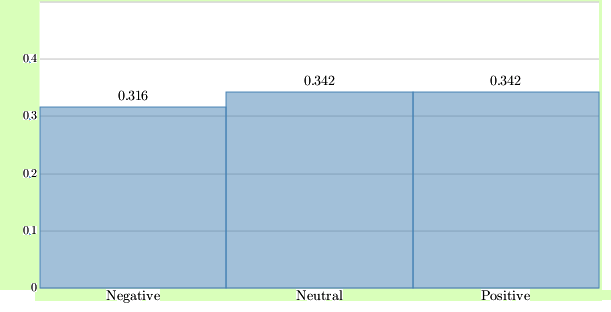
\includegraphics[scale=0.4]{pics/Histogram-HIT1.eps}}
	\caption{Overview of HIT results: distribution of the three categories used in HIT1.}
	\label{distr1}
  \end{center}
\end{figure*}

In order to get an overview of distribution of the results of each HIT, a histogram was plotted for each different task. Figure \ref{distr1} shows a uniform distribution of the three categories used in the simple categorization scheme of HIT1, as could be expected from a balanced dataset.

\begin{figure*}[h]
  \begin{center}
    \fbox{
    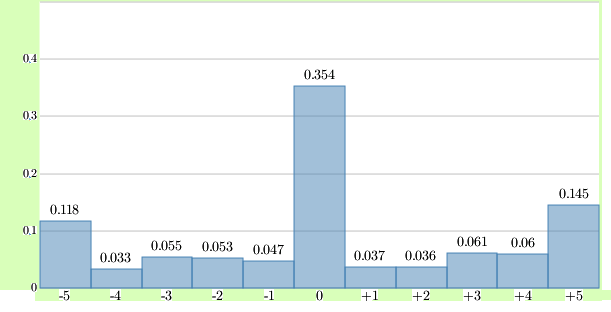
\includegraphics[scale=0.4]{pics/Histogram-HIT2.eps}}
	\caption{Overview of HIT results:  distribution of results in the scaled format of HIT2.}
	\label{distr2}
  \end{center}
\end{figure*}

Figure \ref{distr2} shows the distribution of the graded categorization template of HIT2. Compared to the distribution in \ref{distr1}, two observations can be made: (i) the proportion of the zero values is almost identical to the proportion of the neutral category in Figure \ref{distr1}, and (ii) the proportion of the sum of the positive values [+1,+5] and the proportion of the sum of the negative values [-5,-1] are equally similar to the proportion of the positive and negative categories in \ref{distr1}. This suggests that in order to map the graded annotations of HIT2 to the categories of HIT1, an intuitive partitioning of the graded scale into three equal parts should be avoided. Instead, a more adequate alternative would consist of mapping [-5,-1] to \textit{negative}, 0 to \textit{neutral} and [+1,+5] to \textit{positive}. This means that even slightly positive/negative grades correspond to positive/negative categories.



\begin{figure*}[h]
  \begin{center}
    \fbox{
    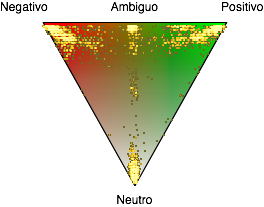
\includegraphics[scale=0.4]{pics/Heatmap-HIT3.eps}}
	\caption{Heat map of the distribution of results in the HIT3 triangle .}
	\label{distr3}
  \end{center}
\end{figure*}

Figure \ref{distr3} (top) shows a heat map that plots the distribution of the annotations in the triangle of HIT3. It appears that worker annotations show a spontaneous tendency of clustering, despite the continuous nature of the design. This suggests that this HIT design, originally conceived as continuous, was transformed by the workers as a simpler categorization task using five labels: \textit{negative}, \textit{ambiguous} and \textit{positive} at the top, \textit{neutral} at the bottom, and \textit{other} in the center.

\begin{figure*}
  \begin{center}
    \fbox{
    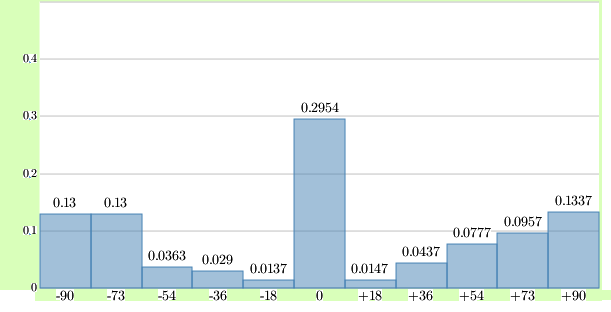
\includegraphics[scale=0.4]{pics/Histogram-HIT3x.eps}}
	\caption{Overview of HIT results: distribution of projection of triangle data points onto the X-axis (positive/negative).}
	\label{distr3b}
  \end{center}
\end{figure*}

% Although the negative-positive axis has been used in some degree as an scale, the other edges, the negative-neutral and the positive-neutral are empty.

Figure \ref{distr3b} shows the distribution of all datapoints in the triangle of Figure \ref{distr3b}, projected onto the X-axis (positive/negative). Although similar to the graded scale in HIT2, the distribution shows a slightly higher polarization.

These results suggest that, out of all three HIT designs, HIT2 is the one that contains the best balance between the amount of information that can be obtained and the simplicity of a one-dimensional annotation. 

%%It could be that the conceptual complexity of a bidimensional annotation would force the annotators to re-interpret the grading task as a classification task.


\subsection{Annotation Quality}
\label{sect:quality}

The annotation quality of AMT workers can be measured by comparing them to expert annotations. This is usually done by calculating inter-annotator agreement (ITA) scores. Note that, since a single HIT can contain more than one assignment and each assignment is typically performed by more than one annotator, we can only calculate ITA scores between batches of assignments, rather than between individual workers. Therefore, we describe the ITA scores in terms of batches. In Table \ref{tablita}, we present a comparison of standard kappa\footnote{In reality, we found that fixed and free margin Kappa values were almost identical, which reflects the balanced distribution of the dataset.} calculations \cite{eugenio_kappa_2004} between batches of assignments in HIT1 and expert annotations.

We found an inter-batch ITA score of 0.598, which indicates a moderate agreement due to fairly consistent annotations between workers. When comparing individual batches with expert annotations, we found similar ITA scores, in the range between 0.628 and 0.649. This increase with respect to the inter-batch score suggests a higher variability among AMT workers than between workers and experts. 
In order to filter out noise in worker annotations, we applied a simple majority voting procedure in which we selected, for each sentence in HIT1, the most voted category. This results in an additional batch of annotations. This batch, refered in Table \ref{tablita} as \textit{Majority}, produced a considerably higher ITA score of 0.716, which confirms the validity of the majority voting scheme to obtain better annotations.

\begin{table}[h]
\begin{center}
\begin{tabular}{|l|c|c|}
\hline
& $\kappa_{1}$ & $\kappa_{2}$ \\ 
\hline
Inter-batch & 0.598 & 0.598 \\ \hline
Batch\_1 vs. Expert & 0.628 & 0.628\\
Batch\_2 vs. Expert & 0.649 & 0.649\\
Batch\_3 vs. Expert & 0.626 & 0.626\\ \hline
Majority vs. Expert & 0.716 & 0.716\\ \hline
Experts\footnote{Results on a different 500-sentence random sample of the same corpus.} & 0.725 & 0.729\\ \hline
\end{tabular}
\end{center}
\label{tablita}
\caption{Interannotation Agreement as a measure of quality of the annotations in HIT1. $\kappa_{1} = $ Fixed Margin Kappa. $\kappa_{2} = $ Free Margin Kappa.}
\end{table}


In addition, we calculated ITA scores between three expert annotators on a separate, 500-sentence dataset, randomly selected from the same corpus as described at the start of Section \ref{sect:design}. This collection was later used as test set in the experiments described in Section \ref{sect:classifier}. The inter-expert ITA scores on this separate dataset contains values of 0.725 for $\kappa_{1}$ and 0.729 for $\kappa_{2}$, only marginally higher than the \textit{Majority} ITA scores. Although we are comparing results on different data sets, these results seem to indicate that multiple AMT annotations are able to produce a similar quality to expert annotations. This might suggest that a further increase in the number of HIT assignments would outperform expert ITA scores, as was previously reported in~\cite{snow_cheap_2008}.
\begin{enumerate}
\item Interannotator agreement depending on the annotator. GOAL: evaluate the annotator reliability
\item Evaluate the bias for the 3 annotators that did most of the work.
\end{enumerate}



\subsection{KAPPA FOR HIT2 and HIT3 using projections to HIT1}



\subsection{Annotation Costs}
\label{sect:costs}

As explained in Section \ref{sect:design}, a total amount of 9000 assignments were uploaded on AMT. At a reward of .02\$ per assignment, a total sum of 225\$ (180\$ + 45\$ Amazon fees) was spent on the task. Workers perceived an average hourly rate of 6.5\$/hour for HIT1 and 8\$/hour for HIT2 and HIT3. These figures suggest that, at least for assignments of type HIT2 and HIT3, a lower reward/assignment might have been considered. This would also be consistent with the recommendations of \cite{mason_financial_2009}, who claim that lower rewards might have an effect on the speed at which the task will be completed - more workers will be competing for the task at any given moment - but not on the quality. Since we were not certain whether a large enough crowd existed with the necessary skills to perform our task, we explicitly decided not to try to offer the lowest possible price.

An in-house expert annotator (working at approximately 70\$/hour, including overhead) finished a batch of 1000 HIT assignments in approximately three hours, which leads to a total expert annotator cost of 210\$. By comparing this figure to the cost of uploading $3 \times 1000$ HIT assignments (75\$), we saved $210 - 75 = 135$\$, which constitutes almost 65\% of the cost of an expert annotator. These figures do not take into account the costs of preparing the data and HIT templates, but it can be assumed that these costs will be marginal when large data sets are used. Moreover, most of this effort is equally needed for preparing data for in-house annotation.



%\section{Supervised polarity classification using Annotations on Mechanical Turk}



\section{Experimental framework: description of datasets}
\label{datasets}

As was mentioned in Section \ref{sect:design}, all sentences were extracted from a corpus of user opinions on cars from the automotive section of \texttt{www.ciao.es} (Spanish). For conducting the experimental evaluation, the following datasets were used:

\begin{enumerate}
\item Baseline: constitutes the dataset used for training the baseline or reference classifiers in Experiment 1. 
Automatic annotation for this dataset was obtained by using the following naive approach: those sentences extracted from
comments with ratings\footnote{The corpus at \texttt{www.ciao.es} contains consumer opinions marked with a score between 1 (negative) and 5 (positive).} equal to 5 were assigned to category `positive', those extracted from comments with ratings 
equal to 3 were assigned to `neutral', and those extracted from comments with ratings equal to 1 were assigned to
`negative'. This dataset contains a total of 5570 sentences, with a vocabulary coverage of 11797 words. 

\item AMT Annotated: constitutes the dataset that was manually annotated by AMT workers in HIT1.
This dataset is used for training the contrastive classifiers which are to be compared with the baseline system in Experiment 1.  It is also used in various ways in Experiment 2. 
The three independent annotations generated by AMT workers for each sentence within this dataset were consolidated into one unique annotation
by majority voting: if the three provided annotations happened to be
different\footnote{This kind of total disagreement among annotators occurred only in 13 sentences out of 1000.}, 
the sentence was assigned to category `neutral'; otherwise, the sentence was assigned to the category with
at least two annotation agreements. This dataset contains a total of 1000 sentences, with a vocabulary coverage 
of 3022 words. 

\item Expert Annotated: this dataset contains the same sentences as the AMT Annotated one, but with annotations produced internally by known reliable annotators\footnote{While annotations of this kind are necessarily somewhat subjective, these annotations are guaranteed to have been produced in good faith by competent annotators with an excellent understanding of the Spanish language (native or near-native speakers)}.  Each sentence received one annotation, while the dataset was split between a total of five annotators.

\item Evaluation: constitutes the gold standard used for evaluating the performance of classifiers.
This dataset was manually annotated by three experts in an independent manner. The gold standard annotation
was consolidated by using the same criterion used in the case of the previous dataset\footnote{In this case, 
annotator inter-agreement was above 80\%, and total disagreement among annotators occurred only in 1 sentence
out of 500}. This dataset contains a total of 500 sentences, with a vocabulary coverage of 2004 words.    
\end{enumerate} 

These three datasets were constructed by randomly extracting sample sentences from an original corpus
of over 25000 user comments containing more than 1000000 sentences in total. The sampling was conducted 
with the following constraints in mind: (i) the three resulting datasets should not overlap, (ii) only sentences 
containing more than 3 tokens are considered, and (iii) each resulting dataset must be balanced, as much
as possible, in terms of the amount of sentences per category. Table \ref{tc_corpus} presents the
distribution of sentences per category for each of the three considered datasets.  

\begin{table}
\begin{center}
\begin{tabular}{|l|l|l|l|}
\hline
&Baseline &Annotated &Evaluation \\
\hline
Positive &1882 &341 &200 \\
\hline
Negative &1876 &323 &137 \\
\hline
Neutral &1812 &336 &161 \\
\hline
Totals &5570 &1000 &500 \\
\hline
\end{tabular}
\caption{Sentence-per-category distributions for baseline, annotated and evaluation datasets.}
\label{tc_corpus}
\end{center}
\end{table}

\section{Experiments}
\label{sect:classifier}


This section intends to evaluate the incidence of AMT-generated annotations on a polarity classification task. We present two different evaluations. In section \ref{eval1}, we compare the results of training a polarity classification system with noisy available metadata and with AMT generated annotations of HIT1. In section \ref{eval2}, we compare the results of training several polarity classifiers using different training sets, comparing expert annotations to those obtained with AMT.


\subsection{Experiment one: AMT annotations vs. original Ciao annotations}
\label{eval1}
A simple SVM-based supervised classification approach was considered for the
polarity detection task under consideration. According to this, two different groups of classifiers were 
used: a baseline or reference group, and a contrastive group. Classifiers within these two groups were
trained with data samples extracted from the baseline and annotated datasets, respectively. Within each group 
of classifiers, three different binary classification subtasks were considered: positive/not\_positive, 
negative/not\_negative and neutral/not\_neutral. All trained binary classifiers were evaluated by computing 
precision and recall for each considered category, as well as overall classification accuracy, over the 
evaluation dataset.

A feature space model representation of the data was constructed by considering the standard bag-of-words approach. 
In this way, a sparse vector was obtained for each sentence in the datasets. Stop-word removal was not
conducted before computing vector models, and standard normalization and TF-IDF weighting schemes were used.

Multiple-fold cross-validation was used in all conducted experiments to tackle with statistical variability of the 
data. In this sense, twenty independent realizations were actually conducted for each experiment presented and,
instead of individual output results, mean values and standard deviations of evaluation metrics are reported.

Each binary classifier realization was trained with a random subsample set of 600 sentences extracted from 
the training dataset corresponding to the classifier group, i.e. baseline dataset for reference systems, 
and annotated dataset for contrastive systems. Training subsample sets were always balanced with respect to 
the original three categories: `positive', `negative' and `neutral'.

%\subsubsection{Results and discussion}

Table \ref{tc_accu} presents the resulting mean values of accuracy for each considered subtask 
in classifiers trained with either the baseline or the annotated dataset. As observed in the table,
all subtasks benefit from using the annotated dataset for training the classifiers; however, it is 
important to mention that while similar absolute gains are observed for the `positive/not\_positive' 
and `neutral/not\_neutral' subtasks, this is not the case for the subtask `negative/not\_negative', 
which actually gains much less than the other two subtasks.

\begin{table}
\begin{center}
\begin{small}
\begin{tabular}{|l|l|l|}
\hline
classifier &baseline &annotated \\ 
\hline
positive/not\_positive &59.63 (3.04) &69.53 (1.70) \\ 
\hline
negative/not\_negative &60.09 (2.90) &63.73 (1.60) \\ 
\hline
neutral/not\_neutral &51.27 (2.49) &62.57 (2.08) \\ 
\hline
\end{tabular}
\end{small}
\caption{Mean accuracy over 20 independent simulations (with standard deviations provided in parenthesis) 
for each classification subtasks trained with either the baseline or the annotated dataset.}
\label{tc_accu}
\end{center}
\end{table}

After considering all evaluation metrics, the benefit provided by human-annotated data 
availability for categories `neutral' and `positive' is evident. However, in the case of category `negative', although some 
gain is also observed, the benefit of human-annotated data does not seem to be as much as for the two other 
categories. This, along with the fact that the `negative/not\_negative' subtask is actually the best performing
one (in terms of accuracy) when baseline training data is used, might suggest that low rating comments contains 
a better representation of sentences belonging to category `negative' than medium and high rating comments do with
respect to classes `neutral' and `positive'. 

In any case, this experimental work only verifies the feasibility of constructing training datasets for
opinionated content analysis, as well as it provides an approximated idea of costs involved in the generation
of this type of resources, by using AMT.


\subsection{Experiment two: AMT annotations vs. expert annotations}
\label{eval2}

In this section, we compare the results of training several polarity classifiers on six different training sets, each of them generated from the AMT annotations of HIT1. The different training sets are: (i) the original dataset of 1000 sentences annotated by experts (\textit{Experts}), (ii) the first set of 1000 AMT results (\textit{Batch1}), (iii) the second set of 1000 AMT results (\textit{Batch2}), (iv) the third set of 1000 AMT results (\textit{Batch3}), (v) the batch obtained by majority voting between Batch1, Batch2 and Batch3 (\textit{Majority}), and (vi) a batch of 3000 training instances obtained by aggregating Batch1, Batch2 and Batch3 (\textit{All}).  We used classifiers as implemented in Mallet \cite{mccallum} and Weka \cite{weka}, based on a simple bag-of-words representation of the sentences.  As the objective was not to obtain optimum performance but only to evaluate the differences between different sets of annotations, all classifiers were used with their default settings.

Table \ref{table:amtvsexp} contains results of four different classifiers (Maxent, C45, Winnow and SVM), trained on these six different datasets and evaluated on the same 500-sentence test set as explained in Section \ref{datasets}.  Classification using expert annotations usually outperforms classification using a single batch (one annotation per sentence) of annotations produced using AMT.  Using the tree annotations per sentence available from AMT, all classifiers reach similar or better performance compared to the single set of expert annotations, at a much lower cost (as explained in section \ref{sect:costs}).

It is interesting to note that most classifiers benefit from using the full 3000 training examples (1000 sentences with 3 annotations each), which intuitively makes sense as the unanimously labeled examples will have more weight in defining the model of the corresponding class, whereas ambiguous or unclear cases will have their impact reduced as their characteristics are attributed to various classes.

On the contrary, Support Vector Machines show an important drop in performance when using multiple annotations, but perform well when using the majority vote.  As a first intuition, this may be due to the fact that SVMs focus on detecting class boundaries (and optimizing the margin between classes) rather than developing a model of each class.  As such, having the same data point appear several times with the same label will not aid in finding appropriate support vectors, whereas having the same data point with conflicting labels may have a negative impact on the margin maximization.

Having only evaluated each classifier (and training set) once on a static test set it is unfortunately not possible to reliably infer the significance of the performance differences (or determine confidence intervals, etc.).  For a more in-depth analysis it might be interesting to use bootstrapping or similar techniques to evaluate the robustness of the results.

\begin{table}
\begin{center}
\begin{small}
\begin{tabular}{|l|l|l|l|l|l|l|} \hline
 System & 
 {\begin{sideways}\parbox{2cm}{\centering Experts}\end{sideways}} &
 {\begin{sideways}\parbox{2cm}{\centering Batch1}\end{sideways}} &
 {\begin{sideways}\parbox{2cm}{\centering Batch2}\end{sideways}} &
 {\begin{sideways}\parbox{2cm}{\centering Batch3}\end{sideways}} &
 {\begin{sideways}\parbox{2cm}{\centering Majority}\end{sideways}} &
 {\begin{sideways}\parbox{2cm}{\centering All}\end{sideways}} \\ \hline
 Winnow & 44.2 & 43.6 & 40.4 & 47.6 & 46.2 & \textbf{50.6} \\ \hline
 SVM & \textbf{57.6} & 53.0 & 55.4 & 54.0 & 57.2 & 52.8 \\ \hline
 C45 & 42.2 & 33.6 & 42.0 & 41.2 & 41.6 & \textbf{45.0} \\ \hline
 Maxent & \textbf{59.2} & 55.8 & 57.6 & 54.0 & 57.6 & 58.6 \\ \hline
\end{tabular}
\end{small}
\end{center}
\caption{Accuracy figures of four different classifiers (Winnow, SVM, C45 and Maxent) trained on six different datasets (see text for details).}
\label{table:amtvsexp}
\end{table}





\subsection{Experiment three: comparative experiments}

\begin{enumerate}
\item Add classification experiments (discret/continuous) using HIT2 annotations
\item Add classification experiments (discret/continuous) using HIT3 annotations

\item Comparative evaluation of classification systems trained with the 3 different HITS (using only the turkers' annotations)
\end{enumerate}

\section{Conclusions}
\label{sect:conclusions}


In this paper we have examined the usefulness of non-expert annotations on Amazon's Mechanical Turk to annotate the polarity of Spanish consumer comments. We discussed the advantages/drawbacks of three different HIT designs, ranging from a simple categorization scheme to a continous scoring template. We report high inter-annotator agreement scores between non-experts and expert annotators and show that training an Opinion Mining System with non-expert AMT annotations outperforms original noisy annotations and obtains competitive results when compared to expert annotations using a variety of classifiers. In conclusion, we found that, in our case, the use of non-expert annotations through crowdsourcing is a viable and cost-effective alternative to the use of expert annotations.

In the classification experiments reported in this paper, we have relied exclusively on AMT annotations from HIT1. \textbf{Further work is needed to fully analyze the impact of each of the HIT designs for Opinion Mining tasks. We hope that the added richness of annotation of HIT2 and HIT3 will enable us to use more sophisticated classification methods.}

\bibliographystyle{naaclhlt2010}
\bibliography{amturk}

\end{document}
